\documentclass[12pt]{report}
\usepackage[T2A]{fontenc}
\usepackage[utf8]{inputenc}
\usepackage[english,russian]{babel}
\usepackage{amssymb,amsfonts,amsmath,mathtext, amsthm}
\usepackage{url, hyperref}
\usepackage{graphicx}
\usepackage{xfrac}

\renewcommand{\L}{\mathcal L}
\newcommand{\F}{\mathcal F}
\newcommand{\R}{\mathbb R}
\renewcommand{\C}{\mathbb C}
\newcommand{\rd}{\mathrm d}
\renewcommand{\i}{i}

\newtheorem{thm}{Теорема}
\newtheorem{rmk}{Замечание}

\title{Тема 2. Операционное исчисление. Преобразование Лапласа.}

\begin{document}
	\maketitle
	\tableofcontents
	
	
\section{Определение}
Преобразованием Лапласа называется отображение вида~\cite{Dubkov:Lecture}
\[
\L : f(t) \mapsto F(p),
\]
где $f(t) \in \F(\R, \C)$, $p = s + \i\sigma \in \C$, такое, что
\[
\L[f(t)]\equiv TF[f(t)] = F(p) = \int_{0}^{\infty} e^{-pt}f(t)\rd t.
\]
$f(t)$ называется \emph{оригиналом}, а $F(p)$ его \emph{изображением по Лапласу}. Пишут:
\[
f(t) \risingdotseq F(p), \text{ и } F(p) \fallingdotseq f(t). 
\]
\paragraph{Ограничения на функцию $f(t)$:}
\begin{enumerate}
	\item $\forall t < 0f(t) \equiv 0$. Это условие всегда можно полагать верным при решении задач Коши.
	\item $\forall t > 0,~ f(t)$ на каждом конечном сегменте области определения имеет только конечное число разрывов первого рода, а в остальных точках удовлетворяет условию Липшица-Гельднера: 
	\[\exists\tau_0>0\forall \tau \leq \tau_0 |f(t+\tau) - f(t)| \leq A|\tau|^\alpha.\]
	Любая непрерывно-дифференцируемая функция удовлетворяет этому условию.
	\item $f(t)$ растёт не быстрее показательной функции: \[ |f(t)| < Me^{p_0t}.\] Это всегда справедливо для физических процессов.
\end{enumerate}

\paragraph{Обратное преобразование}
\[
f(t) = \L^{-1}[F(p)] = \frac{1}{2\pi\i}\int_{a - \i\infty}^{a+\i\infty}e^{pt}F(p)\rd p, ~ a\in\R.
\]

\section{Свойства~\cite{Dubkov:Lecture}}
\begin{enumerate}
	\item Линейность.
	\[
	\forall\alpha,\beta\in\C\left[\alpha f(t)\beta g(t) \risingdotseq \alpha F(p) + \beta G(p)\right]
	\]
	Следствие линейности интеграла.
	\item Теорема подобия.
	\[
	\forall\alpha>0 \left[f(\alpha t) \risingdotseq \frac 1\alpha F\left(\frac p\alpha\right) \right].
	\]
	(Заменить $\alpha t = \tau$ в интеграле.)
	\item Теорема запаздывания.
	\[
	f(t-\tau) \risingdotseq e^{-p\tau} F(p).
	\]
	Поскольку $f(t-\tau) \equiv 0$, $\int_0^\infty \to \int_\tau^\infty$; $\tau < t < \infty$, 
	$0 < \underbrace{t-\tau}_{\theta} < \infty$, $t = \theta + \tau$.
	\item Теорема смещения.
	\[
	e^{p_0t} f(t) \risingdotseq F(p-p_0).
	\]
	\item Дифференцирование оригинала. $f\in C^n$ \label{itm:prop-diff-original}
	\begin{align*}
	f'(t) &\risingdotseq p F(p) - f(+0), \\
	&\dots \\
	f^{(n)}(t) &\risingdotseq p^nF(p) -\sum_{k=0}^{n-1}p^{n-1-k}f^{(k)}(+0).
	\end{align*}
%	где $f^{(k)}(0) = \lim_{t \to +0} f^{(k)}(t)$.
	\item Дифференцирование изображения.
	\[
	F^{(n)}(p) \fallingdotseq (-t)^nf(t).
	\]
	\item  Интегрирование оригинала.
	\[
	\int_0^t f(\tau)\rd\tau \risingdotseq \frac 1p F(p).
	\]
	\item Интегрирование изображения.
	\[
	\int_p^\infty F(q)\rd q \fallingdotseq \frac 1t f(t).
	\]
	\item Предельные теоремы.
	\begin{align*}
		\lim\limits_{p\to \infty} pF(p) &= f(0),\\
		\lim\limits_{p\to0} pF(p) &= f(\infty) \equiv \lim_{t\to\infty}f(t).
	\end{align*}
\end{enumerate}

\begin{thm}[Первая теорема разложения]
	Если функция $F(p)$ -- аналитична~\footnote{В окрестности любой точки своей области определения представима сходящимся степенным рядом.} в окрестности $|p|>R$ бесконечно удалённой точки, и имеет в ней разложение в ряд Лорана:
	\[
	F(p) = \sum_{n=1}^{\infty}\frac{c_n}{p^n},
	\]
	то её оригинал:
	\[
	f(t) = \sum_{n=1}^{\infty}\frac{c_n}{(n-1)!}t^{n-1}.
	\]
\end{thm}

\begin{rmk}
	Существует вторая теорема разложения, в~\cite[стр.~27]{Dubkov:Lecture} можно её почитать. 
	Также, на 26-й странице пример применения первой теоремы разложения при решении задачи.
\end{rmk}

\begin{thm}[Планшереля]
	Пусть $f_1,f_2 \in L^2$ (квадратично-интегрируемые функции), $g_1(u), g_2(u)$ -- их преобразования Фурье. Тогда верно:
	\[
	\int_{-\infty}^{+\infty} g_1(u)g_2(u)\rd u = \int_{-\infty}^{+\infty} f_1(x)f_2(-x)\rd x.
	\]
	
	В упрощённой форме:
	\[
	\int_{-\infty}^{+\infty} |\F\{x(t)\}|^2\rd w = \int_{-\infty}^{+\infty}|x(t)|^2\rd t;
	\]
	физическая интерпретация~\cite[после~ф-лы~8]{Plancherel}: \emph{энергия колебательного сигнала равна сумме энергий его гармонических компонент.}
\end{thm}

\section{Свёртка (convolution)}
Свёрткой называется:
\begin{align*}
f(t)\otimes g(t) &= \int_{-\infty}^{+\infty} f(\tau)g(t-\tau)\rd\tau \\
&= \int_{-\infty}^{+\infty} g(\tau)f(t-\tau)\rd\tau.
\end{align*}

\begin{rmk}
	Характерным для свёртки является наличие аргумента $t-\tau$ у одной из функций (границы интеграла могут быть и другие).
\end{rmk}

\begin{thm}[о свёртке\label{thm:convolution}]
	\[
	f(t)\otimes g(t)\risingdotseq F(p)\cdot G(p).
	\]
\end{thm}

\paragraph{Интеграл Дюамеля}
\begin{figure}[h]\centering
	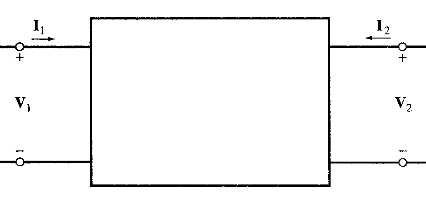
\includegraphics[width=\linewidth]{quadripole}
	\caption{Линейный четырёхполюсник с переходной характеристикой $h(t)$.\label{fig:quadripole}}
\end{figure}

В радиотехнике (см. Рис.~\ref{fig:quadripole})
\[
V_2(t) = \int_0^t h(t-\tau)V_1(\tau)\rd \tau = h(t)\otimes V_1(t).
\]

\begin{figure}[h]\centering
	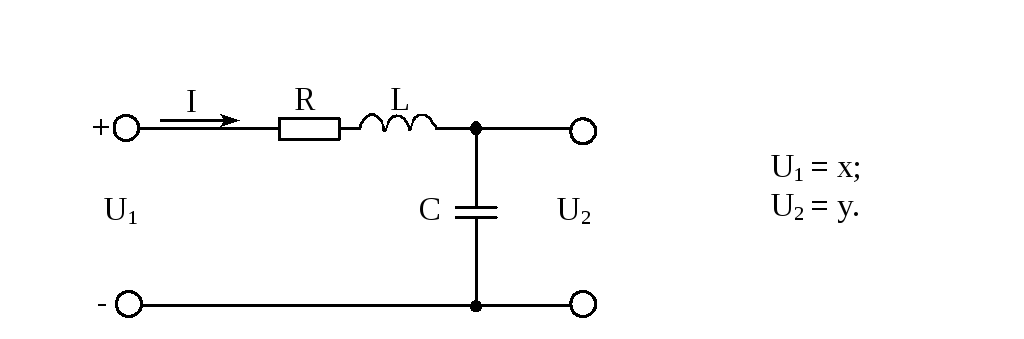
\includegraphics[width=\linewidth]{RLC_quadripole}
	\caption{RLC-четырёхполюсник.\label{fig:RLC-quadripole}}
\end{figure}

Где удобно использовать операционное исчисление? Для решения электротехнических задач. В цепочке из Рис.~\ref{fig:RLC-quadripole}:
\begin{align*}
	u &= Ri, \tag{R-элемент} \\
	u &= L\frac{\rd i}{\rd t}, \tag{L-элемент} \\
	i &= C\frac{\rd u}{\rd t}. \tag{C-элемент}
\end{align*}

Можно было бы записать:
\begin{align*}
	U_1 &= U_R + U_L + \underbrace{U_C}_{U_2}, \\
	U_1 &= iR + L\frac{\rd i}{\rd t} + \frac1C\int i\rd t.
\end{align*}

А можно представить L-/C-элементы как реактивное сопротивление, и использовать делитель напряжения:
\begin{align*}
	U_2(p) &= K(p)U_1(p), \\
	K(p) &= \frac{\sfrac{1}{pC}}{pL + R + \sfrac{1}{pC}},
\end{align*}
$K(p)$ -- коэффициент передачи.

\section{Связь с преобразованием Фурье}
Фурье-образ (или частотный спектр функции)
\[
F(\i\omega)  =\F[f(t)]= \int_{-\infty}^{+\infty}f(t)e^{-\i\omega t}\rd t.
\]
\paragraph{Условия существования преобразования Фурье~\cite{Fourier-conditions}}
\begin{enumerate}
	\item $f(t)$ однозначная функция, с конечным числом минимумов, максимумов, и разрывов;
	\item Условие абсолютной интегрируемости: $\int_{-\infty}^{+\infty}|f(t)|\rd t < \infty$.
\end{enumerate}

\emph{Пример.} $\int_{-\infty}^{+\infty} |1(t)| \rd t \to \infty$, поэтому у этой функции нет Фурье-образа.

Что можно сделать в этом случае? 

Домножить $f(t)$ на $e^{-st}$, чтобы интеграл получившегося произведения сходился.
Но если так сделать, получим 
\begin{align*}
F(s,\i\omega) &= \int_{-\infty}^{+\infty}f(t)e^{-st}e^{-\i\omega t}\rd t, ~ p = s + \i\omega  \\
&= \int_{-\infty}^0 f(t) e^{-pt}\rd t + \int_0^{+\infty} f(t) e^{-pt}\rd t \\
&= \int_0^{+\infty} f(-t) e^{-p(-t)}\rd t + \int_0^{+\infty} f(t) e^{-pt}\rd t \\
&= \L[f(-t); -p] + \L[f(t); p] = \L_B[f(t)].
\end{align*}
Последнее равенство -- двустороннее преобразование Лапласа; таким образом, непрерывное преобразование Фурье эквивалентно двустороннему преобразованию Лапласа.

\section{Задачи}
\subsection{Дифференциальные уравнения}
В задачах по теме присутствуют задачи Коши, которые надо решить используя операционное исчисление. Как это делать объяснено в ~\cite{difur}. В целом, ничего сложного, надо просто: 
\begin{enumerate}
	\item Используя теорему о дифференцировании оригинала~\ref{itm:prop-diff-original} (и таблицу преобразований для элементарных функций) записать алгебраическое уравнение для изображений. На этом шаге используется тот факт, что нам даны начальные условия -- это позволяет исключить символ $f^{(k)}(+0)$.
	\item Выразить образ искомой функции в виде дроби. В числителе и знаменателе дроби -- многочлены от $p$, и знаменатель хорошо бы разложить на множители; это упростит следующий шаг.
	\item Теперь,  чтобы произвести обратное преобразование, нужно разложить получившуюся дробь в сумму простых дробей. Для этого используется метод неопределённых коэффициентов.~\cite{indefinite-coef-method}
	\item Когда решение для образа функции представлено суммой простых дробей, производим обратное преобразование Лапласа. 
\end{enumerate}

\subsection{Интегральные уравнения}
Последняя задача -- интегральное уравнение. Если быть точным, перед нами уравнение Вольтерра второго рода.~\cite[см.~ф-лу~8.11]{integral-equations} Там можно заметить интеграл типа ``свёртки'' $\int_0^t g(t-\tau)x(\tau)\rd\tau$ (аргумент одной из функций $t-\tau$).

Чтобы его решить, надо применить теорему~\ref{thm:convolution} (о свёртке), получить алгебраическое уравнение для образов, разрешить его относительно образа искомой функции, по возможности упростить получившуюся дробь, и произвести обратное преобразование Лапласа.

\begin{thebibliography}{0}
	\bibitem{Dubkov:Lecture}
	А.А. Дубков, Н.В. Агудов. Преобразование Лапласа. Учебно-методическое пособие.
	\url{http://www.lib.unn.ru/students/src/Laplace%20transform.pdf}
	\bibitem{Fourier-conditions}
	Преобразование Фурье.
	\url{http://drive.ispu.ru/elib/lebedev/2.html}
	\bibitem{Plancherel}
	Фурье преобразование.
	\url{https://www.booksite.ru/fulltext/1/001/008/117/965.htm}
	\bibitem{difur}
	Как решить дифференциальное уравнение
	методом операционного исчисления?
	\url{http://mathprofi.ru/reshenie_diffurov_metodom_operacionnogo_ischislenija.html}
	\bibitem{indefinite-coef-method}
	Интегрирование дробно-рациональной функции. 
	Метод неопределенных коэффициентов
	\url{http://mathprofi.ru/integraly_ot_drobno_racionalnoj_funkcii.html}
	\bibitem{integral-equations}
	Интегральные урванения типа ``свёртки.''
	\url{https://studfiles.net/preview/6312517/page:9/}
\end{thebibliography}
\end{document}